\documentclass[tikz,border=6pt]{standalone}
\usepackage[utf8]{inputenc}
\usepackage[T1]{fontenc}
\usepackage{amsmath,amssymb}
\usepackage{pgfplots}
\pgfplotsset{compat=1.18}
\usepgfplotslibrary{groupplots}

\begin{document}
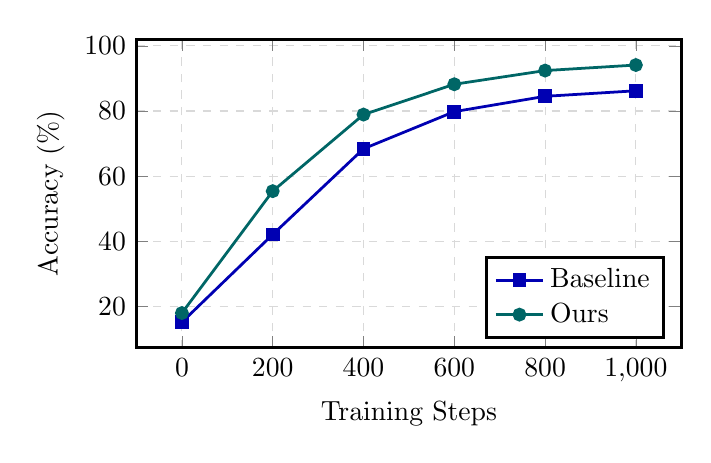
\begin{tikzpicture}
\begin{axis}[
    width=8.5cm,
    height=5.5cm,
    grid=major,
    grid style={dashed, gray!30},
    xlabel={Training Steps},
    ylabel={Accuracy (\%)},
    legend pos=south east,
    legend cell align={left},
    line width=1pt
]

\addplot[color=blue!70!black, mark=square*] coordinates {
    (0, 15.2) (200, 42.1) (400, 68.4) (600, 79.8) (800, 84.5) (1000, 86.2)
};
\addlegendentry{Baseline}

\addplot[color=teal!80!black, mark=*] coordinates {
    (0, 18.0) (200, 55.4) (400, 78.9) (600, 88.2) (800, 92.4) (1000, 94.1)
};
\addlegendentry{Ours}

\end{axis}
\end{tikzpicture}
\end{document}
